%%%%%%%%%%%%%%%%%%
% Based on https://github.com/jdavis/latex-homework-template
%%%%%%%%%%%%%%%%%%

\documentclass{article}

\usepackage{fancyhdr}
\usepackage{extramarks}

\usepackage{amsmath}
\usepackage{amsthm}
\usepackage{amsfonts}

\usepackage{tikz}
\usepackage[plain]{algorithm}
\usepackage{algpseudocode}

\usetikzlibrary{automata,positioning}

\usepackage{wrapfig}

\usepackage{lipsum}

%for urls
\usepackage{hyperref}
\hypersetup{
	colorlinks = true,
	linkcolor = teal,
	anchorcolor = teal,
	citecolor = teal,
	filecolor = teal,
	urlcolor = teal
}

%%%%%% Basic Document Settings %%%%%%%%%

\topmargin=-0.45in
\evensidemargin=0in
\oddsidemargin=0in
\textwidth=6.5in
\textheight=9.0in
\headsep=0.25in

\linespread{1.1}

%%%%%%%%%%%%%%%%%% Homework Details %%%%%%%%%%%%%%%
% University Logo
% Title
% Due date
% University
% Class
% Instructor
% Author
% Author ID 
\newcommand{\hmwkSeal}{images/logo.png}
\newcommand{\hmwkTitle}{Pac-man Projects Contest (Phase C)}
\newcommand{\hmwkDueDate}{Jan 24, 2023}
\newcommand{\hmwkClass}{Introduction to Artificial Intelligence (CS-487) }
\newcommand{\hmwkClassInstructor}{Professor I. Tsamardinos}
\newcommand{\hmwkUniversity}{University of Crete \\Department of Computer Science}
\newcommand{\hmwkAuthorName}{Nikolaos-Modestos Kougioulis}
\newcommand{\hmwkAuthorID}{ID 1285}


%fancyhdr
\pagestyle{fancy}
\lhead{\hmwkAuthorName\ (\hmwkAuthorID)} %left head
%\chead{\hmwkClass\ \hmwkTitle} %center head
%\rhead{\date{\today}} %right head
\rhead{\hmwkTitle} 
\lfoot{\lastxmark}
\cfoot{\thepage}

\renewcommand\headrulewidth{0.4pt}

% Create Problem Sections %

\newcommand{\enterProblemHeader}[1]{
	\nobreak\extramarks{}{Problem \arabic{#1} continued on next page\ldots}\nobreak{}
	\nobreak\extramarks{Problem \arabic{#1} (continued)}{Problem \arabic{#1} continued on next page\ldots}\nobreak{}
}

\newcommand{\exitProblemHeader}[1]{
	\nobreak\extramarks{Problem \arabic{#1} (continued)}{Problem \arabic{#1} continued on next page\ldots}\nobreak{}
	\stepcounter{#1}
	\nobreak\extramarks{Problem \arabic{#1}}{}\nobreak{}
}

\setcounter{secnumdepth}{0}
\newcounter{partCounter}
\newcounter{exerciseCounter}
\setcounter{exerciseCounter}{1}
\nobreak\extramarks{Problem \arabic{exerciseCounter}}{}\nobreak{}

% Homework Problem Environment %
% This environment takes an optional argument. When given, it will adjust the problem counter. This is useful for when the problems given for your
% assignment aren't sequential. See the last 3 problems of this template for an example.
%

\newenvironment{Exercise}[1][-1]{
	\ifnum#1>0
	\setcounter{exerciseCounter}{#1}
	\fi
	\section{Exercise \arabic{exerciseCounter}}
	\setcounter{partCounter}{1}
	\enterProblemHeader{exerciseCounter}
}{
	\exitProblemHeader{exerciseCounter}
}

% Title Page %
\title{
	\centering
	\includegraphics[height=1.5in]{\hmwkSeal}
	
	\vspace{1in}
	\textmd{\textbf{\hmwkClass\ \hmwkTitle}}\\
	
	\normalsize\vspace{0.1in}\small{Due\ on\ \hmwkDueDate}\\
	
	\vspace{0.1in}
	\large{\textit{\hmwkClassInstructor}} \\
	\vspace{0.5in}
	
	\large{\hmwkUniversity}
	
	\vspace{3in}
	
	\author{\textbf{\hmwkAuthorName} (\hmwkAuthorID)}
	\date{\today}
}

% Various Helpers %
\newcommand{\alg}[1]{\textsc{\bfseries \footnotesize #1}}
% For derivatives
\newcommand{\deriv}[1]{\frac{\mathrm{d}}{\mathrm{d}x} (#1)}
% For partial derivatives
\newcommand{\pderiv}[2]{\frac{\partial}{\partial #1} (#2)}
% Integral dx
\newcommand{\dx}{\mathrm{d}x}
\newcommand{\E}{\mathbb{E}}
\newcommand{\Var}{\mathrm{Var}}
\newcommand{\Cov}{\mathrm{Cov}}
\newcommand{\Bias}{\mathrm{Bias}}

\def\code#1{\texttt{#1}}

%for code listings
\usepackage{listings}
\usepackage{xcolor}

\definecolor{codegreen}{rgb}{0,0.6,0}
\definecolor{codegray}{rgb}{0.5,0.5,0.5}
\definecolor{codepurple}{rgb}{0.58,0,0.82}
\definecolor{backcolour}{rgb}{0.99,0.99,0.99}

\lstdefinestyle{mystyle}{
	backgroundcolor=\color{backcolour},   
	commentstyle=\color{codegreen},
	keywordstyle=\color{magenta},
	numberstyle=\tiny\color{codegray},
	stringstyle=\color{codepurple},
	basicstyle=\ttfamily\footnotesize,
	breakatwhitespace=false,         
	breaklines=true,                 
	captionpos=b,                    
	keepspaces=true,                 
	numbers=left,                    
	numbersep=5pt,                  
	showspaces=false,                
	showstringspaces=false,
	showtabs=false,                  
	tabsize=2
}

\lstset{style=mystyle}

\begin{document}
	
	\maketitle
	
	\pagebreak
	
	\section{Introduction}
	
	For Phase C of the Pac-Man Projects we are asked to create an agent that successfully competes and solves the original map of Pac-Man (available with the argument \code{-l originalClassic}), in the form of competition with fellow students. The implementation should not be laggy and require an extensive amount of time to complete (such as looping back and forth to finite states), as well as being advised to make use of the Expectimax agent that was created for the needs of Phase B of the Projects. \\
	
	We combine properties of the Expectimax, FoodSearch and Reflex agents to create a new agent called the \textit{Hybrid Agent}, that consistently wins high scoring games in a time-efficient manner. \\
	
	\tableofcontents
	\listoffigures
	
	\newpage
	
	\section{Methods - The \textit{HybridAgent} class}
	
	In this section we introduce a new agent class to solve the task of the project. Before coming up with a non-naive and trivial approach to the problem of solving the \textit{originalClassic} map, we must make the following assumptions:
		
	\begin{itemize}
		\item \textbf{Assumption 1:} If implementing Expectimax, always assume depth 3. This derives from the test command provided in  the guidelines\footnote{we are recommended to test our implementation by running \code{pacman.py -p ExpectimaxAgent -a depth=3 -l originalClassic}}. 
		\item \textbf{Assumption 2:} We are not restricted to a single agent behavior but may apply collection of agent behaviors to a single agent, hereon called the \textit{Hybrid Agent}.
		\item \textbf{Assumption 3:} Assume we can evaluate the performance of the hybrid agent by comparing against an average human player (and surely not against Billy Mitchell).
	\end{itemize}
	
	\vspace{10pt}
	For our implementation, we follow an approach similar to what an average human player would follow. By average we refer to an individual familiar with the rules and goals of Pac-Man, but not knowledgeable with how each individual ghost behaves and which actions prove optimal in the long run, maximizing the final score. We use the following three rules: \\
	
	\textbf{Rule 1:} If the closest distance to a ghost is over $k$, then find the optimal path from the current position to the closest food pellet. That is, if the following is satisfied
	
	$$ \text{min} \left( \left\{ d_{\text{M}} (x_p, x_i), ~i=1,2,3 \right\} \right) > k \Rightarrow \text{min} \left( \left\{ | x^1_p - x^1_i | + | y^1_p - y^2_i|, ~i=1,2,3 \right\} \right) > k$$
	
	proceed with a food pellet searching algorithm, where $x_i$ are the three adversarials of Pac-Man: Blinky (red), Inky (cyan), Pinky (pink) and Clyde (orange). \\
	
	\textbf{Rule 2:} If the closest distance to a ghost is at most $k$, then perform Expectimax assuming a uniform distribution for the adversarials' actions. \\
	
	\textbf{Rule 3:} In case a food pellet is unreachable, handle illegal actions by randomly being a left turn only or right turn only agent. \\
	\begin{figure}[h]
		\centering
		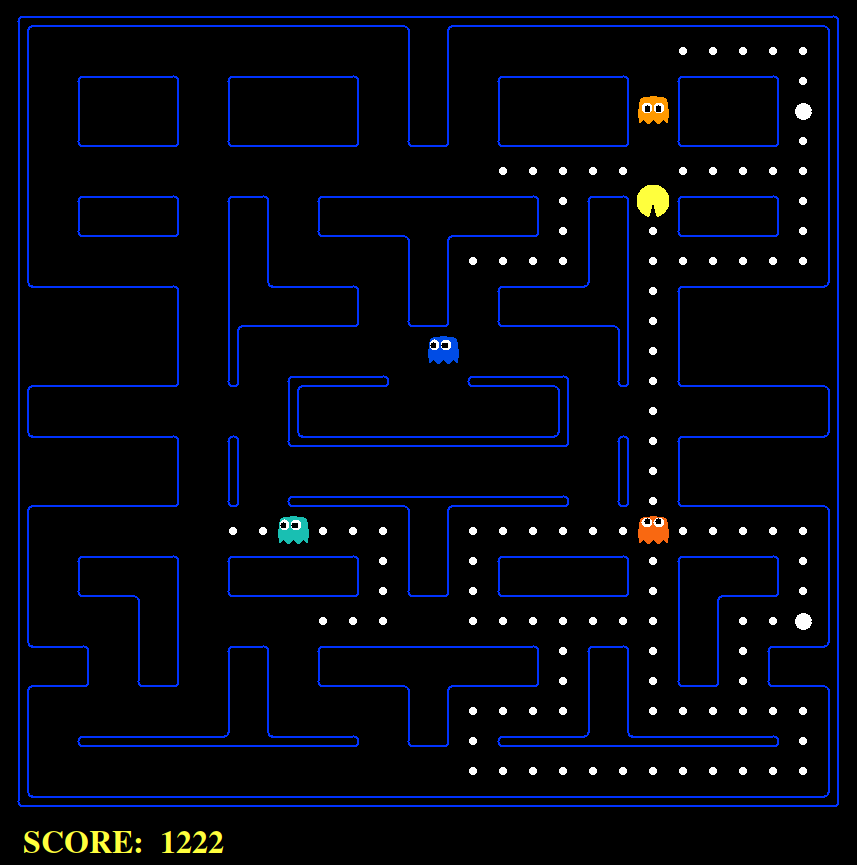
\includegraphics[width=0.4\textwidth]{images/gameplay.png}
		\caption{Gameplay of the Pac-Man Projects on \textit{originalClassic} map. The screenshot illustrates our \textit{HybridAgent} mid-game.}
		
	\end{figure}

	We define \textit{HybridAgent} as the agent combining the above three rules. The intuition behind this implementation is simple: If ghosts are far from Pac-Man, then they do not pose a realistic threat, so it is sensible to ignore them altogether and focus on collecting the most amount of food pellets. However when ghosts get close to Pac-Man to a constant $k$, then Pac-Man can sense death is near and uses Expectimax to avoid the ghosts while collecting as much food pellets as possible. The evaluation function has also been altered a bit in order to eat a scared ghost when eating a power capsule(by returning $+\infty$ as score) and run away from certain death (by returning $-\infty$ as score). \\
	
	The path to the nearest food pellet is obtained using Breadth-First Search: At each step of the game we obtain the coordinates of Pac-Man and then proceed to get the coordinates of each legal action. This is better illustrated with the following code snippet:
	
	\begin{lstlisting}[language=Python]
	#use Breadth-First Search to find the path to the closest food
	
	startingNode = curr_pos 
	queue = util.Queue()
	visited = set() #use dictionary for faster lookup
		
	queue.push((startingNode, []))
	
	if curr_pos == closest_food:
	    return []
		
	#return the first action that leads to the closest food
	while not queue.isEmpty():
		node, path = queue.pop()
		if node not in visited:
		    visited.add(node)
		if node == closest_food:
		    print("Path to follow:", path)
		    return path[0]
		for action in legal:
		    if action == Directions.STOP:
		        continue	
		    #get coordinates of the next nodes in the path
		    if action == Directions.NORTH:
		        successor = (node[0], node[1] + 1)
		    elif action == Directions.SOUTH:
		        successor = (node[0], node[1] - 1)
		    elif action == Directions.WEST:
		        successor = (node[0] - 1, node[1])
		    elif action == Directions.EAST:
		        successor = (node[0] + 1, node[1])
		    elif action == Directions.STOP:
		        successor = node
		    #if none of the above, then the action is not valid
		    else:
		        continue
		    if successor not in visited and successor not in walls:
		        queue.push((successor, path + [action]))		
	\end{lstlisting}

Full code of the DFS implementation and the HybridAgent class is available in the appendix of this document, as well on the associated python source file. 
\newpage

\section{Results}

As per guidelines, \textit{HybridAgent} is run on the \textit{originalClassic} layout 10 times. The scores of each game, the average score and win rate is shown in Figure 2. We implement our HybridAgent using $k=4$. The scores of 10 human played game instances are illustrated in Figure 3. \\

\textit{Our HybridAgent wins all 10 games, with a $\code{3112.9}$ average score, while for the human player 2 are lost.} \\

To compare the human player with HybridAgent, we perform the Wilcoxon Signed-rank test, a non-parametric statistical test, for sample size $n=10$. For each instance, we compute the difference between the two scores $D_i$. We then obtain the absolute values $|D_1|, |D_2|$, \ldots $|D_n|$ and order them from smallest to largest by assigning them ranks from $1$ to $n$, $r(|D_1|), ~r(|D_2|), \ldots, r(|D_n|)$. We also keep a record of the original signs of the differences, notating $I^+$ and $I^-$ the list of indices $i$ for which the signs were positive and negative respectively. The Wilcoxon statistic $W$ is the smallest of $W^+$ (the sum of the positive ranks) and $W^-$ (the sum of the negative ranks),


$$W = \text{min}(W^+, W^-) = \text{min} (\sum_{i \in I^+} r(|D_i|), \sum_{i \in I^-} r(|D_i|) )$$

which does not depend on the distribution of the samples (hence non-parametric). For large $n$, the W-statistic converges to the normal distribution. The null hypothesis is $\text{H}_0 : P(X_\alpha) > P(X_\beta) = 1/2$, that is, a randomly chosen observation from the first group is equally probable of being larger than a randomly drawn observation from the second group. Performing a two-tailed test, we obtain a mean difference $-283.1$, sum of positive ranks $W^+ =37$ and sum of negative ranks $W^- = 18$. The Wilcoxon test-statistic is therefore $W = 18$. The critical value of $W$, obtained from a table of critical values for $n = 10$ and $\alpha=0.05$ is $8$. Since $W > 8$ we do not have statistically significant evidence to reject then null hypothesis. Hence the results are not statistically significant, so we can assume our HybridAgent performs as well as the average human player.

\begin{figure}[h]
	\centering
	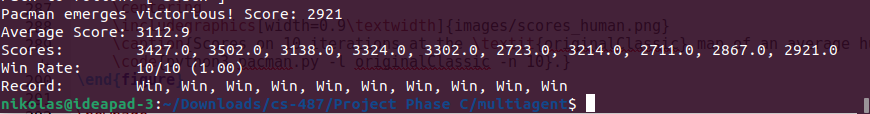
\includegraphics[width=0.9\textwidth]{images/scores.png}
    \caption{Scores on 10 iterations at the \textit{originalClassic} map of our \textit{HybridAgent}, by running \code{python3 pacman.py -p HybridAgent -a depth=3 -l originalClassic -n 10}.}
    	 
\end{figure}

\begin{figure}[h]
	\centering
	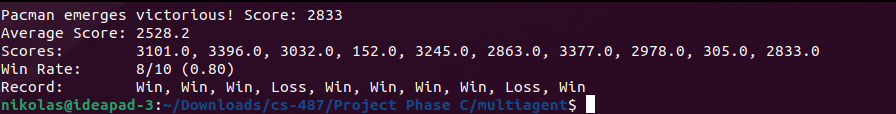
\includegraphics[width=0.9\textwidth]{images/scores_human.png}
	\caption{Scores on 10 iterations at the \textit{originalClassic} map of an average human player, running \code{python3 pacman.py -l originalClassic -n 10}.}
\end{figure}

\newpage

\section{Discussion}

One computational improvement on the above implementation is to replace Breadth-First Search with an informed search algorithm, such as uniform-cost search or A-star search. \\

Ideally in larger maps, one can implement Markov Decision Processes with rewards. At each time step, the Markov process is in some state $s$ and associates each action $a$ resulting in a new state $s'$ with a reward $R_a(s,s')$. These processes, as the name suggests, satisfy the Markov property known from Markov chains: the next state $s'$ depends only on the current state $s$ and the action $a$.   

\newpage

\section{Appendix}

\appendix

	\begin{lstlisting}[language=Python, caption=The HybridAgent class]
class HybridAgent(MultiAgentSearchAgent):
	"""
	Hybrid Agent
	"""
	
	def getAction(self, gameState):
	
	    #for pacman
	    def max_value(gameState, depth):
	        legalActions = gameState.getLegalActions(0)
	        if not legalActions or depth == self.depth:
	            return self.evaluationFunction(gameState)
	        v = float("-inf")
	        v = max(exp_value(gameState.generateSuccessor(0, action), 0 + 1, depth + 1) for action in legalActions)
	        return v
	
	    #for all ghosts
	    def exp_value(gameState, agentIndex, depth):
	        legalActions = gameState.getLegalActions(agentIndex)
	        if not legalActions:
	            return self.evaluationFunction(gameState)
	
	        prob = 1.0 / len(legalActions)
	        v = 0
	        for action in legalActions:
	            newState = gameState.generateSuccessor(agentIndex, action)
	            if agentIndex == gameState.getNumAgents() - 1:
	               v += max_value(newState, depth) * prob
	            else:
	               v += exp_value(newState, agentIndex + 1, depth) * prob
	        return v
	
	     ghostPositions = gameState.getGhostPositions()
	     distanceToGhost = [util.manhattanDistance(gameState.getPacmanPosition(), ghost) for ghost in ghostPositions]
	
		 if(min(distanceToGhost) > 4):
	
	       curr_pos = gameState.getPacmanPosition()
	       foods = gameState.getFood().asList() #list of food coordinates
	       capsules = gameState.getCapsules() #list of capsule coordinates
	       walls = gameState.getWalls().asList()
	       #closest food coordinate
	       closest_food = min(foods, key=lambda x: util.manhattanDistance(curr_pos, x))
	
	       legal = gameState.getLegalActions(0)
	
	       #return the action to the closest food dot
	       print("Closest food pellet: ", str(closest_food))
	       print("Legal actions: ", legal)
	
	       #use Breadth-First Search to find the path to the closest food
	       startingNode = curr_pos 
	       queue = util.Queue()
	       visited =  set() #use dictionary for faster lookup
	
	       queue.push((startingNode, []))
	
	       print("Current position: ", str(curr_pos))
	
	       if curr_pos == closest_food:
	           return []
	
	       #return the first action that leads to the closest food
	       while not queue.isEmpty():
	           node, path = queue.pop()
	           if node not in visited:
	               visited.add(node)
	               if node == closest_food:
	                   print("Path to follow:", path)
	                   return path[0]
	               for action in legal:
 	                   if action == Directions.STOP:
	                       continue
	
	                   #get coordinates of the next nodes in the path
	                   if action == Directions.NORTH:
	                       successor = (node[0], node[1] + 1)
	                   elif action == Directions.SOUTH:
	                       successor = (node[0], node[1] - 1)
	                   elif action == Directions.WEST:
	                       successor = (node[0] - 1, node[1])
	                   elif action == Directions.EAST:
	                       successor = (node[0] + 1, node[1])
	                   elif action == Directions.STOP:
	                       successor = node
	                   #if none of the above, then the action is not valid
	                   else:
	                       continue
	                   if successor not in visited and successor not in walls:
	                       queue.push((successor, path + [action]))
	 
	       #handling illegal moves if the closest food is not reachable by becoming a right turn or left turn reflex agent
	       if not gameState.hasFood(gameState.getPacmanPosition()[0] + 1, gameState.getPacmanPosition()[1]) and gameState.hasFood(gameState.getPacmanPosition()[0] - 1, gameState.getPacmanPosition()[1]):
	           legal = gameState.getLegalActions(0)
	           current = gameState.getPacmanState().configuration.direction
	           if current == Directions.STOP: current = Directions.NORTH
	           left = Directions.LEFT[current]
	           if left in legal: return left
	           if current in legal: return current
	           if Directions.RIGHT[current] in legal: return Directions.RIGHT[current]
	           if Directions.LEFT[left] in legal: return Directions.LEFT[left]
	           return Directions.STOP
	       elif not gameState.hasFood(gameState.getPacmanPosition()[0] - 1, gameState.getPacmanPosition()[1]) and gameState.hasFood(gameState.getPacmanPosition()[0] + 1, gameState.getPacmanPosition()[1]):
	           legal = gameState.getLegalActions(0)
	           current = gameState.getPacmanState().configuration.direction
	           if current == Directions.STOP: current = Directions.NORTH
	           right = Directions.RIGHT[current]
	           if right in legal: return right
	           if current in legal: return current
	           if Directions.LEFT[current] in legal: return Directions.LEFT[current]
	           if Directions.RIGHT[right] in legal: return Directions.RIGHT[right]
	           return Directions.STOP
	       else:
	           if random.uniform(0, 1) < 0.5: 
	               legal = gameState.getLegalActions(0)
	               current = gameState.getPacmanState().configuration.direction
	               if current == Directions.STOP: current = Directions.NORTH
	               right = Directions.RIGHT[current]
	               if right in legal: return right
	               if current in legal: return current
	               if Directions.LEFT[current] in legal: return Directions.LEFT[current]
	               if Directions.RIGHT[right] in legal: return Directions.RIGHT[right]
	               return Directions.STOP
	           else:
	               legal = gameState.getLegalActions(0)
	               current = gameState.getPacmanState().configuration.direction
	               if current == Directions.STOP: current = Directions.NORTH
	               left = Directions.LEFT[current]
	               if left in legal: return left
                   if current in legal: return current
	               if Directions.RIGHT[current] in legal: return Directions.RIGHT[current]
	               if Directions.LEFT[left] in legal: return Directions.LEFT[left]
	               return Directions.STOP
	
	   #if a ghost is close, death is near so use Expectimax
		 else:
	       best_action = None
 	       legalActions = gameState.getLegalActions()
	       best_action = max(legalActions, key=lambda action: exp_value(gameState.generateSuccessor(0, action), 1, 1))
	       print("A ghost is close! Performing Expectimax at location:", gameState.getPacmanPosition())
	       return best_action	
\end{lstlisting}

\end{document}
